\section{Appendix}
\appendix

\renewcommand{\thesubsection}{\Alph{subsection}}

\subsection{Gantt Chart}
\label{app:gantt}
\begin{center}
    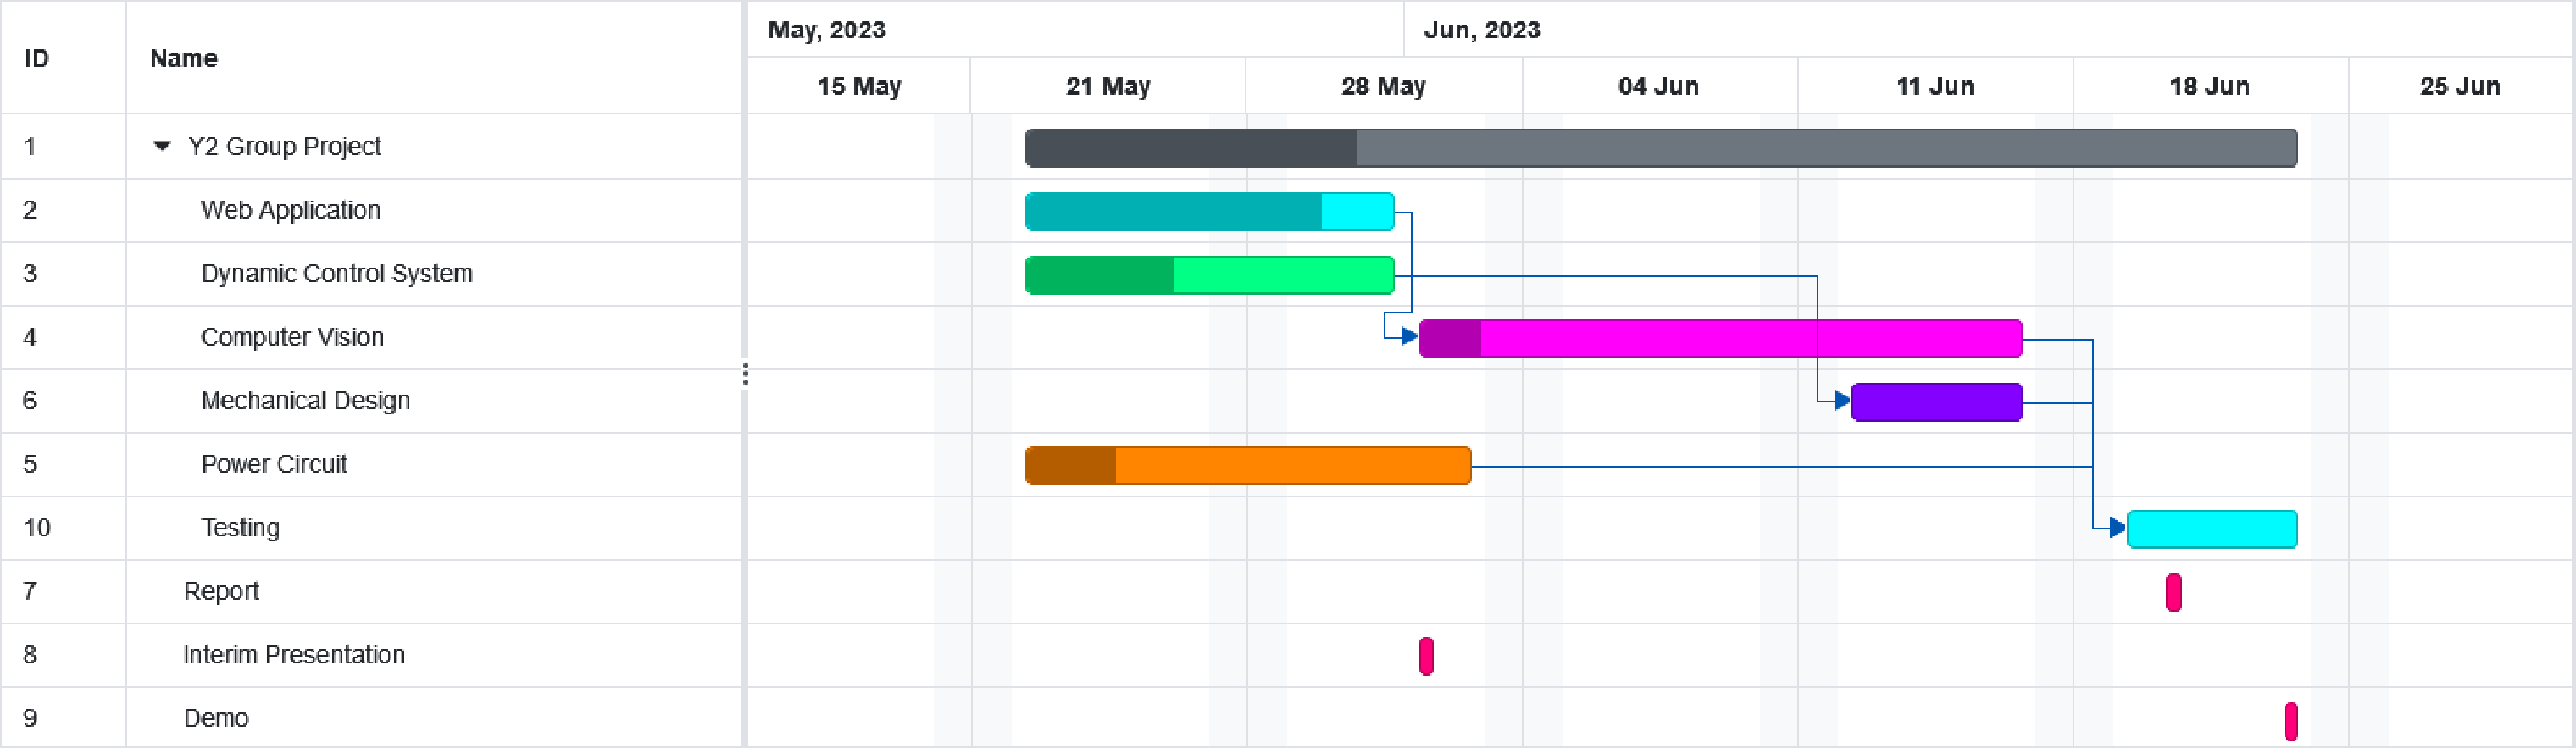
\includegraphics[width=\textwidth]{includes/Y2GanttChartt.pdf}
\end{center}

\subsection{Tilting example}
\begin{center}
    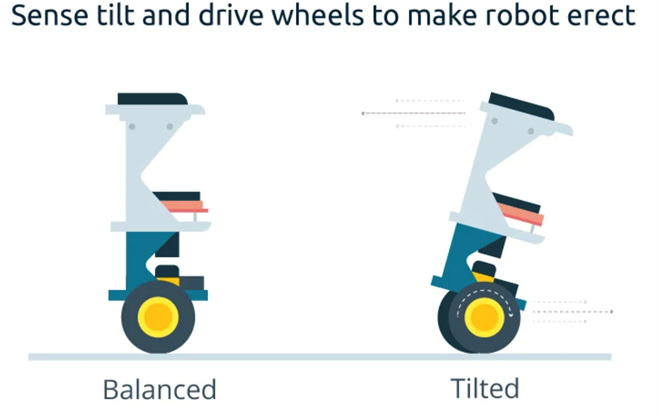
\includegraphics[width=\textwidth]{images/balancing-image.png}
\end{center}

\subsection{ToTal Algorithm}
\label{app:total}
Given the three beacon coordinates \({x_1, y_1}, {x_2, y_2}, {x_3, y_3}\) and the robot coordinates \({x_0, y_0}\), and the three angles \({\alpha_1, \alpha_2, \alpha_3}\):
\begin{enumerate}
    \item Compute the modified beacon coordinates: \\
        \(x'_1 = x_1 - x_2, y'_1 = y_1 - y_2, y'_3 = y_3 - y_2\) \\
    \item compute the three cot: \\
        \(T_{12} = \cot(\alpha_2 - \alpha_1), T_{23} = \cot(\alpha_3 - \alpha_2), T_{31} = \frac{1-T_{12}T_{23}}{T_{12} + T_{23}}\)
    
    \item Compute the modified circle center coordinates: \\
        \(x'_12 = x'1 + T_{12}y'_1, y'_12 = y'_1 - T_{12}x'_1,\) \\
        \(x'_23 = -x'3 - T_{23}y'_3, y'_23 = -y'_3 + T_{23}x'_3,\) \\
        \(x'_31 = (x'_3 + x'_1) + T_{31}(y'_3 - y'_1),\) \\
        \(y'_31 = (y'_3 + y'_1) - T_{31}(x'_3 - x'_1)\) 
    
    \item Compute \(k'_{31}\): \\

        \(k'_{31} = x'_1x'_3 + y'_1y'_3 + T_{31}(x'_1y'_3 - x'_3y'_1)\)
    
    \item Compute D ( if D = 0, return with an error):

        \(D = (x'_{12}-x'_{23})(y'_{23}-y'_{31}) - (y'_{12}-y'_{23})(x'_{23}-x'_{31})\)
    
    \item Compute the robot position \({x_R, y_R}\): \\
        \(x_R = x_2 + \frac{k'_{31}(y'_{12}-y'_{23})}{D}, y_R = y_2 + \frac{k'_{31}(x'_{23}-x'_{12})}{D}\)
\end{enumerate}


\subsection{Control system code}
\label{app:control}
\begin{minted}{arduino}
void keepBalancing() {
  // Read tilt angle from MPU6050
  sensors_event_t a, g, temp;
  mpu.getEvent(&a, &g, &temp);

  // Apply calibration offsets
  float calibratedX = a.acceleration.x - offsetX;
  float calibratedY = a.acceleration.y - offsetY;
  float calibratedZ = a.acceleration.z - offsetZ;

  // Calculate the tilt angle
  float currentAngle = atan2(-calibratedX, 
    sqrt(calibratedY * calibratedY + calibratedZ * calibratedZ)) * 180.0 / PI;

  // Calculate the difference between target and current angle
  float angleError = targetAngle - currentAngle;

  // PID control calculations
  double output = Kp * angleError
                + Ki * integralTerm
                + Kd * (angleError - prevError);

  // Update the integral term
  integralTerm += angleError; 

  // Update the previous error
  prevError = angleError;

  // Adjust motor speeds based on PID output
  if (output > angleThreshold) {
    motor1.setSpeed(motorSpeed);
    motor2.setSpeed(-motorSpeed);
  } else if (output < -angleThreshold) {
    motor1.setSpeed(-motorSpeed);
    motor2.setSpeed(motorSpeed);
  }
  else {
    motor1.setSpeed(0);
    motor2.setSpeed(0);
  }

  // Move the motors
  motor1.runSpeed();
  motor2.runSpeed();
}

void calibrateMPU6050() {
  float sumX = 0.0;
  float sumY = 0.0;
  float sumZ = 0.0;
  const int numSamples = 500;

  // Collect calibration data
  for (int i = 0; i < numSamples; i++) {
    sensors_event_t a, g, temp;
    mpu.getEvent(&a, &g, &temp);
    sumX += a.acceleration.x;
    sumY += a.acceleration.y;
    sumZ += a.acceleration.z;
    delay(10);
  }
  Serial.println("Callibration Complete");

  // Calculate calibration offsets
  offsetX = sumX / numSamples;
  offsetY = sumY / numSamples;
  offsetZ = sumZ / numSamples;
  Serial.print("OffsetX: ");
  Serial.println(offsetX);
  Serial.print("OffsetY: ");
  Serial.println(offsetY);
  Serial.print("OffsetZ: ");
  Serial.println(offsetZ);
}
\end{minted}


\subsection{Datasheet Links}

\begin{itemize}
  \item \textbf{Stepper Motors} -- \url{https://pages.pbclinear.com/rs/909-BFY-775/images/Data-Sheet-Stepper-Motor-Support.pdf}
  \item \textbf{MPU6050} -- \url{https://invensense.tdk.com/wp-content/uploads/2015/02/MPU-6000-Datasheet1.pdf}
  \item \textbf{ESP32} -- \url{https://www.espressif.com/sites/default/files/documentation/esp32-wroom-32d_esp32-wroom-32u_datasheet_en.pdf}
  \item \textbf{D8M} --  \url{https://www.terasic.com.tw/cgi-bin/page/archive_download.pl?Language=English&No=1071&FID=d1a1859ab8be9c1db7d1ecac282badfd}
\end{itemize}